%!TEX root = ../main.tex

\section{Исследование обобщения модели}

\begin{frame}{Постановка задачи}
\vspace{-3mm}
Работа \cite{ponomarev_generalization} \\[2mm]
Исследуем распределение фазового поля вокруг проводников ($\phi = 0$) различного вида. Пусть $\Phi \equiv 0$. Рассмотрим следующие краевые задачи:
\begin{center}
\begin{tabular}{{|%
    >{\raggedright\arraybackslash}m{28mm}|%
    c|%
    c|%
    >{\centering\arraybackslash}m{45mm}|%
}}
    \hline
    &&& \\[-3.5mm]
    Плоский \linebreak случай & $\clOmega = [0, +\infty)_x \times I_y \times J_z$ & $\phi|_{x = 0} = 0$ & $\phi \to 1$ при \linebreak $r = x \to +\infty$ \\[3mm]
    \hline
    &&& \\[-3.5mm]
    Цилиндрический \linebreak случай & $\clOmega = \Real_x \times \Real_y \times J_z$ & $\phi|_{x, y = 0} = 0$ & $\phi \to 1$ при \linebreak $r = \sqrt{x^2 + y^2} \to +\infty$ \\[3mm]
    \hline
    &&& \\[-3.5mm]
    Сферический \linebreak случай & $\clOmega = \Real_x \times \Real_y \times \Real_z$ & $\phi|_{x, y, z = 0} = 0$ & $\phi \to 1$ при \linebreak $r = \sqrt{x^2 + y^2 + z^2} \to +\infty$ \\[3mm]
    \hline
\end{tabular}
\end{center}
Ищем стационарное решение $\phi = \phi(r)$.
\end{frame}


\begin{frame}{Суть проблемы}
\begin{columns}
\column{0.5\textwidth}
    \centering
    Плоский случай
\column{0.5\textwidth}
    \centering
    Цилиндрический случай
\end{columns}
\vspace{0.5cm}
\begin{columns}
\column{0.49\textwidth}
    \hspace{1mm} Задача Коши:
    \vspace{-0.3cm}
    \[
        \phi(0) = 0; \qquad \partr{\phi} = \cfrac{2}{l} \sqrt{1 - f(\phi)}
    \]
    \vspace{-0.3cm}
    \begin{figure}
        
\includegraphics[width=\textwidth]{figures/result_volumes.png}
    \end{figure}
\column{0.01\textwidth}
    \rule{0.4pt}{0.7\textheight}
\column{0.49\textwidth}
    \centering
    Задача поставлена некорректно \\ и решения не имеет \cite{zipunova_higher_codimension}. \\[0.2cm]
    Вместе с тем канал пробоя -- одномерный объект в трехмерном пространстве!
\end{columns}
\end{frame}


\begin{frame}{Обобщение модели}
\vspace{-0.3cm}
\begin{block}{Обобщение модели, предложенное в работе \cite{zipunova_higher_codimension}}
\begin{itemize}
    \item Уравнение фазового поля $\phi$:
    \[
        \cfrac{1}{m} \partt{\phi} = \half \epsilon'(\phi) \gradsq{\Phi} + \cfrac{\Gamma}{l^2} f'(\phi) + \half \Gamma \Delta \phi - \alpha \cfrac{\Gamma l^2}{4} \bilapl{\phi} + \beta \Gamma l^{p - 2} \plapl{\phi}{p - 2}
    \]
    \vspace{-4mm}
\end{itemize}
\end{block}
\begin{itemize}
    \item $\bilapl{\phi} = \Delta(\Delta \phi)$ -- билапласиан
    \item $\plapl{\phi}{p - 2}$ -- $p$-лапласиан
\end{itemize}
\vspace{1mm}
Везде далее $p = 4$.
\end{frame}


\begin{frame}{Разностная схема}
\parind На границе $r = 0$ расчетной области у решения $\phi$ ожидается особенность. \\[3mm]
\parind Идея подхода:
\begin{itemize}
    \item используем метод конечных объемов: к ячейке $\Omega_i$ отнесено среднее $\widetilde{\phi}_i$ функции $\phi$;
    \item в первой и второй ячейках приближаем $\phi$ ЛК базисных функций, \\ одна из которых имеет тот же вид особенности, что решение $\phi$;
    \item как и в классическом МКО, уравнения на $\widetilde{\phi}_i$ являются следствием \\ балансовых соотношений.
\end{itemize}
\end{frame}


\begin{frame}{Полученные результаты}
\vspace{-3mm}
\begin{center}
    Предполагаемые виды особенности решения $\phi$ в точке $r = 0$
\end{center}
\vspace{-1mm}
\begin{tabular}{|m{3cm}||m{3.5cm}|m{3.5cm}|m{3.5cm}|}
    \hline
    &&& \\[-3mm]
    &
    \multicolumn{1}{c}{$\alpha = 0$, $\beta = 0$} &
    \multicolumn{1}{c}{$\alpha = 0$, $\beta \neq 0$} &
    \multicolumn{1}{c}{$\alpha \neq 0$} \\[-2mm]
    &&& \\[-1.5mm]
    \hline
    \hline
    &&& \\[-3.5mm]
    Плоский \linebreak случай & \textcolor{dark_green}{Без особенности} & \textcolor{dark_green}{Без особенности} & \textcolor{dark_green}{Без особенности} \\[3.5mm]
    \hline
    &&& \\[-3.5mm]
    Цилиндрический \linebreak случай & \textcolor{dark_red}{Не имеет решения} & $r^{2/3}$ & $r^2 \ln r$ \\[3.5mm]
    \hline
    &&& \\[-3.5mm]
    Сферический \linebreak случай & \textcolor{dark_red}{Предположительно не имеет решения} & $r^{1/3}$ & \textcolor{dark_red}{Предположительно не имеет решения} \\[3.5mm]
    \hline
\end{tabular}
\begin{itemize}
    \item Базисная функция $g$ подбирается так, чтобы
    \vspace{-0.2cm}
    $$\rho[\phi = g] \cdot S \to C > 0 \text{ при } r \to +0.$$
\end{itemize}
\end{frame}


\begin{frame}{Полученные результаты}
\vspace{-0.5cm}
\begin{figure}
    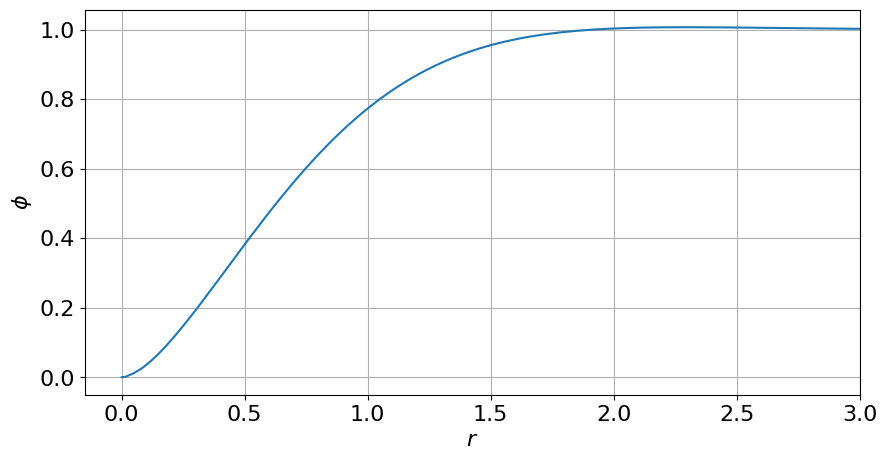
\includegraphics[width=0.81\textwidth]{figures/result_volumes_cyl_bi.png}
\end{figure}
\vspace{-0.7cm}
\begin{center}
    Цилиндрический случай, $\alpha = 1$, $\beta = 0$: особенность вида $r^2 \ln r$
\end{center}
\end{frame}


\begin{frame}{Полученные результаты}
\vspace{-0.5cm}
\begin{figure}
    
\includegraphics[width=0.81\textwidth]{figures/result_volumes_sph_p.png}
\end{figure}
\vspace{-0.7cm}
\begin{center}
    Сферический случай, $\alpha = 0$, $\beta = 1$: особенность вида $r^{1/3}$
\end{center}
\end{frame}